\section{Evaluation}
\label{sec:evaluation}

We present an experimental evaluation of the \projecttitle implementation (\secref{implementation}). The main goal of our evaluation is to measure the provenance overheads imposed by~\projecttitle and quantify the sources for these overheads.

\subsection{Experimental Setup}
We first describe the experimental setup used for the evaluation.

\myparagraph{Experimental platform} We used an Intel Xeon processor based
multicore architecture as our host machine for our evaluation. The
host system consists of 8 cores (16 threads) of Intel(R) Xeon(R) CPU Processor D-1540
(12M Cache, 2.00 GHz) and 32 GB of DRAM main memory. The host
machine is running Linux with kernel 4.2.0 in 64-bit mode.
The GCC 4.9.2 compiler was used to
compile (with -$03$ optimization flag) the benchmark applications.

\myparagraph{Applications and dataset}  For the evaluation, we use the PARSEC~\cite{parsec} and
Phoenix~\cite{phoenix} benchmark suites. We use
the input data and parameters as specified by the
benchmarks. \tabref{overheads} lists the applications used for the
evaluation.

\begin{figure}[h]
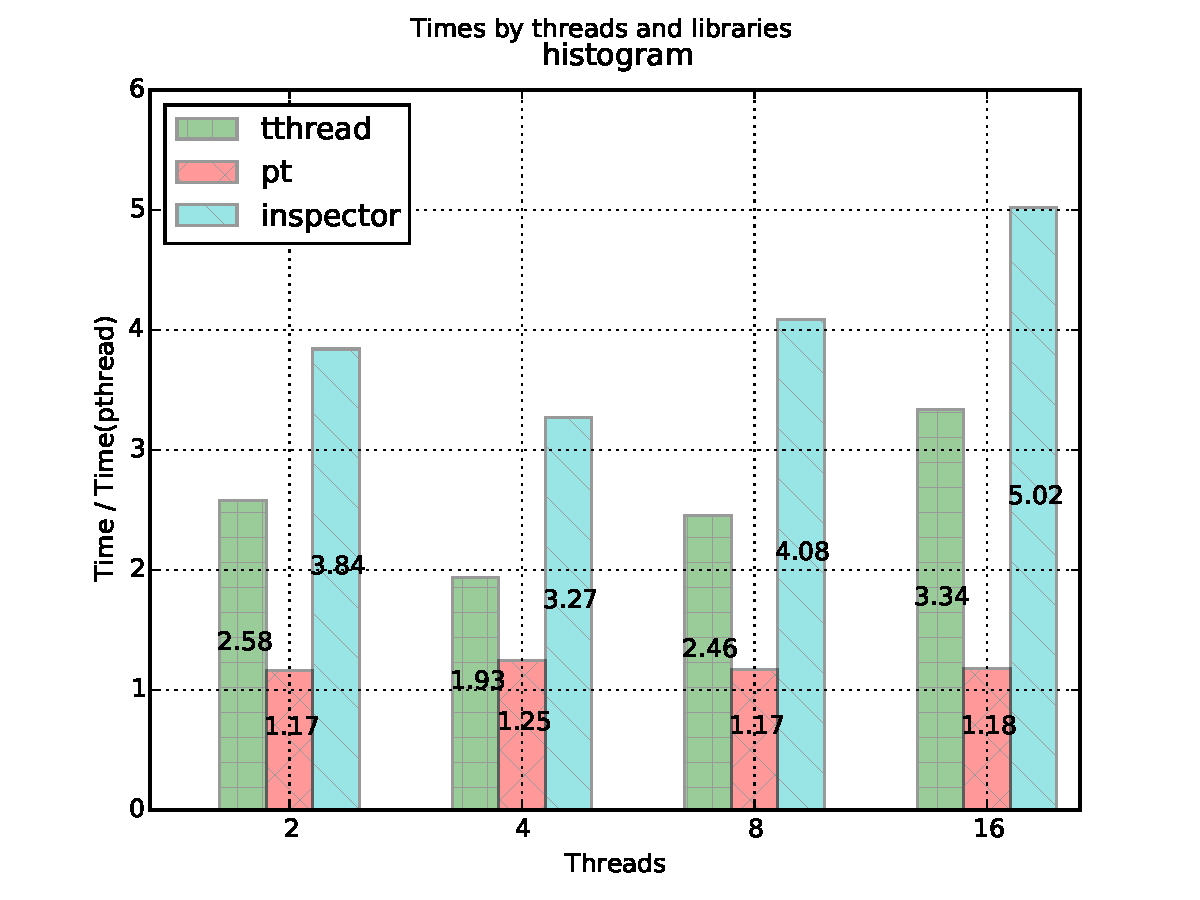
\includegraphics[width=8cm]{figure/histogram.pdf}
\end{figure}

\begin{figure}[h]
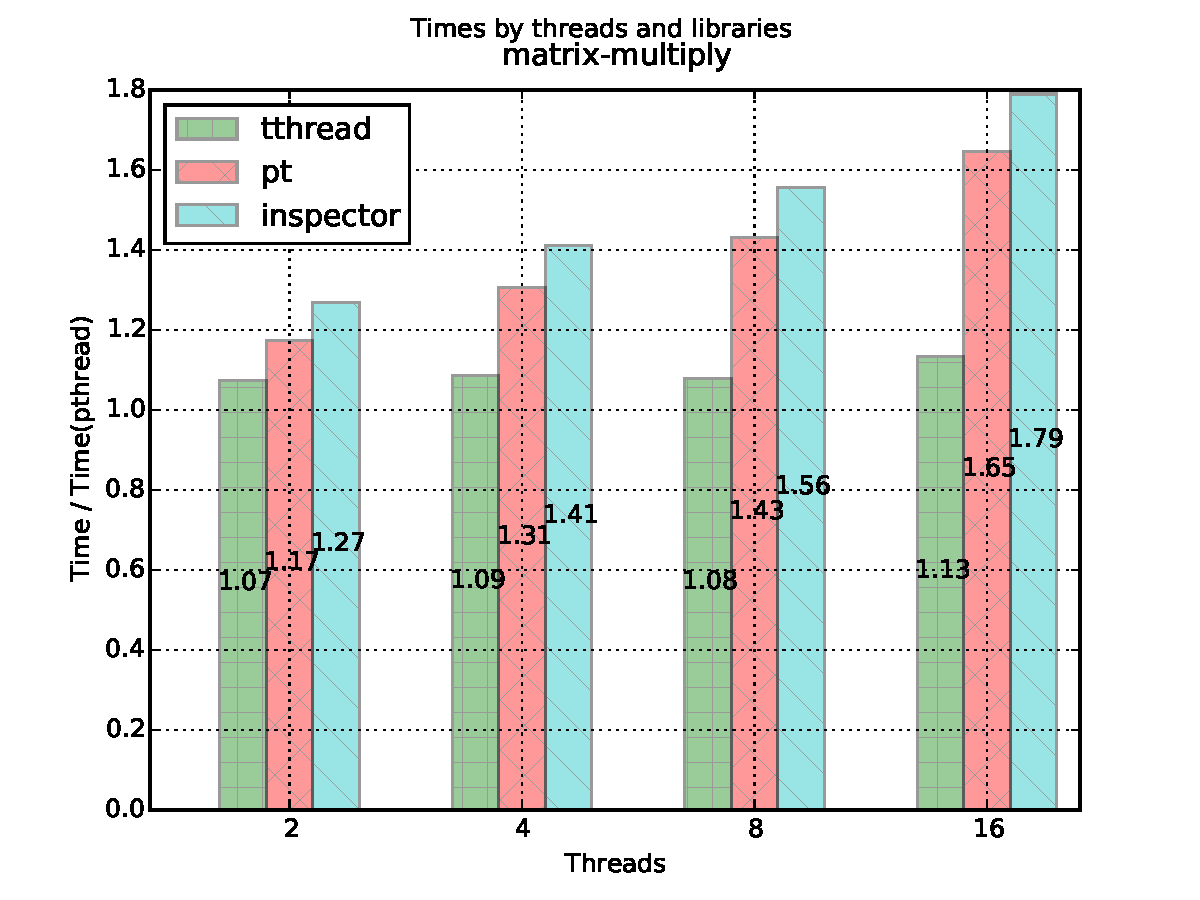
\includegraphics[width=8cm]{figure/matrix-multiply.pdf}
\end{figure}

\begin{figure}[h]
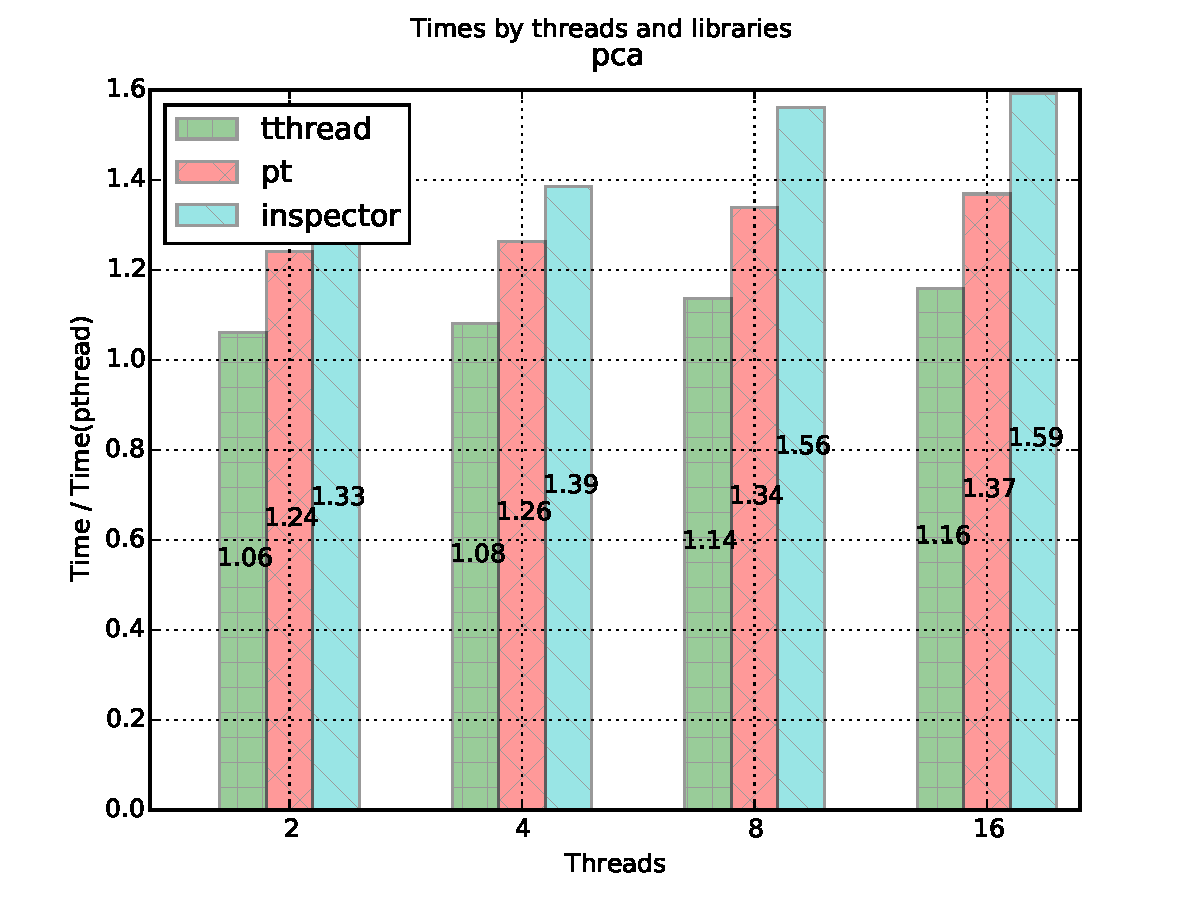
\includegraphics[width=8cm]{figure/pca.pdf}
\end{figure}

\begin{figure}[h]
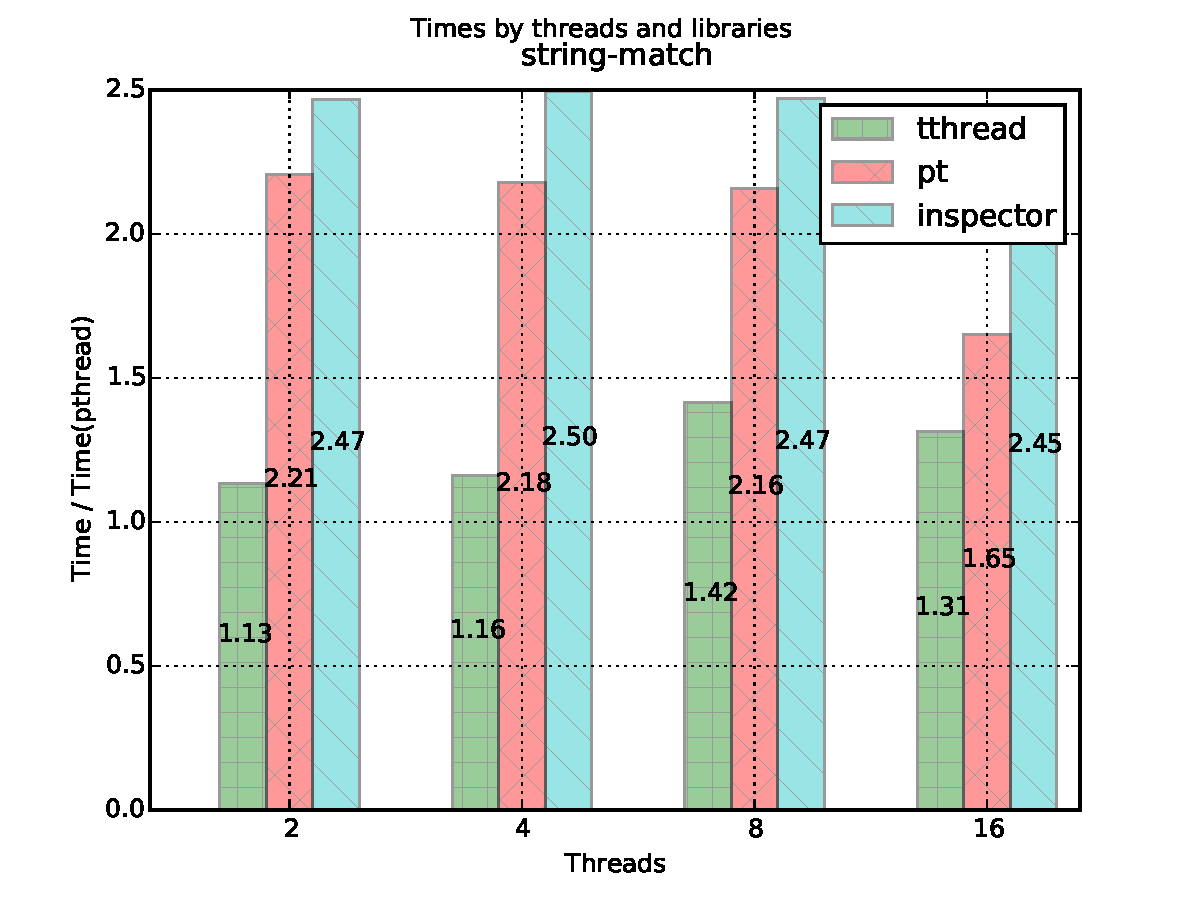
\includegraphics[width=8cm]{figure/string-match.pdf}
\end{figure}

\begin{figure}[h]
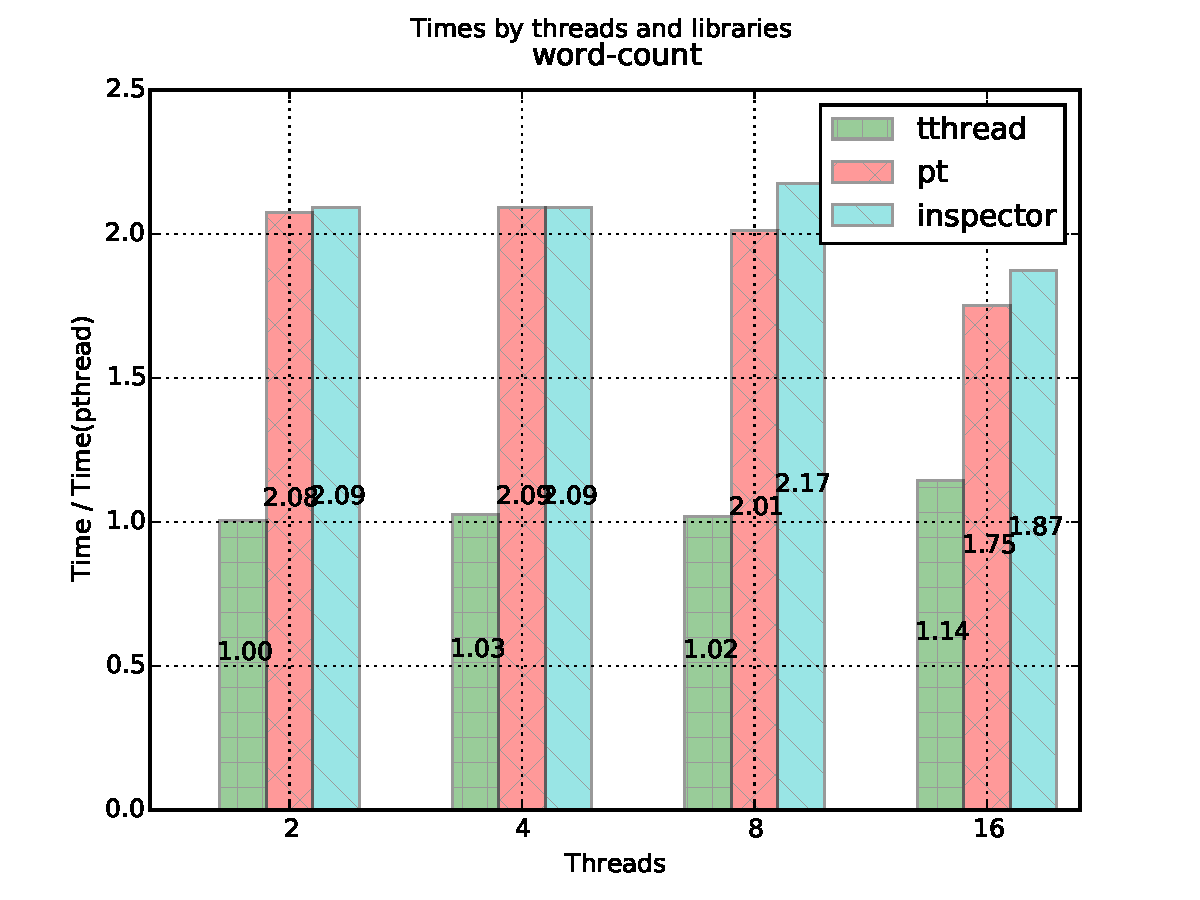
\includegraphics[width=8cm]{figure/word-count.pdf}
\end{figure}

%
%\myparagraph{Performance metrics: Work and Time}  For each run, we consider two types of measures: \emph{work} and
% {\em time}. Work refers to the total amount of
%computation performed by all threads and is measured as the total
%run-time of all threads. Time refers to the amount of (end-to-end)
%run-time to complete the parallel computation. Both metrics are important
%and complementary: time measurements reflect the end user perceived latency,
%whereas work measurements assess the overall resource (CPU) utilization.

\subsection{Provenance Overheads}

\myparagraph{Overheads}

\myparagraph{Breakdown of overheads}

\myparagraph{Overheads w.r.t. input size}
